
\begin{frame}[allowframebreaks, t, fragile]{Artigo 3: Resultados}
  
          
  \begin{figure}[hbt]
    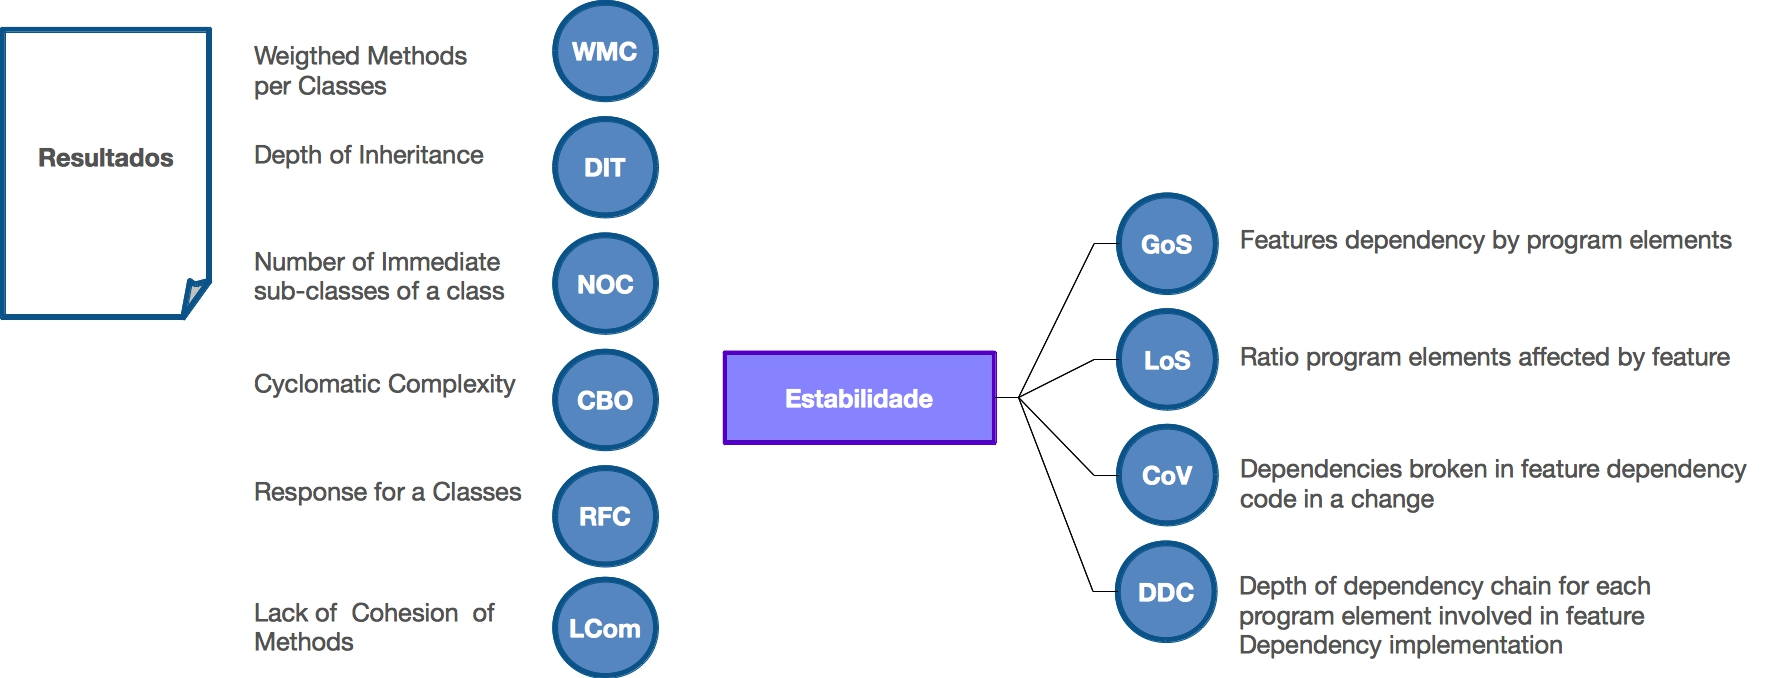
\includegraphics[scale=0.25]{imagens/artigo3-resultados-1.jpg}
  \end{figure}

%   \begin{table}\centering
%      \small
%      \begin{tabular}{@{} p{2cm}  p{8cm} @{}}
%	\toprule
%	  \textbf{Métrica} & \textbf{Descrição}      \\
%	  \midrule
%	  WMC   & Quantidade de operações por classe ou aspecto.\\
%	  DIT	& Profundidade da árvore de herança 	     \\
%	  NOC	& Quantidade de sub-classes ou sub-aspectos em um módulos \\
%	  CBO   & Acoplamento entre interfaces, classes e ou aspectos 	         \\
%	  RFC   & Quantidade de métodos ou advices executados em resposta a uma mensagem recebida.	 \\
%	  LCOM  & Quantidade de pares de operações trabalhando em campos diferentes de classes ou aspectos menos
%	   os pares de operações trabalhando com atributos em comum (Lack de coesão entre métodos)	 \\
%	  \bottomrule
%      \end{tabular}
%   \end{table}
%   
%   \framebreak
%   \begin{table}\centering
%      \small
%      \begin{tabular}{@{} p{2cm}  p{8cm} @{}}
%	\toprule
%	  \textbf{Métrica} & \textbf{Descrição}      \\
%	  \midrule
%    	GoS   & Quantidade de operações por classe ou aspecto.\\
%    	LoS	  & Profundidade da árvore de herança 	     \\
%    	CoV	  & Quantidade de sub-classes ou sub-aspectos em um módulos \\
%    	DDC   & Acoplamento entre interfaces, classes e ou aspectos\\
%	  \bottomrule
%      \end{tabular}
%   \end{table}

\end{frame}